\graphicspath{{chapters/03/images}}
\chapter{Objectives}

\section{Revealing neural correlates of sleep in the olfactory system of the honey bee}
The main objective of this work is to reveal the neural correlates of sleep in the olfactory system of the honeybee.
To do so a computational system of the antennal lobe will be developed and used to simulate the activity of the antennal lobe in both sleep and awake states.
The model will be built based on the work performed on \cite{bee-geosmin} and \cite{data-driven-antennal-lobe-model}.
The parameter of the model will be fine-tuned to match the activity of the antennal lobe recorded in \cite{sleep-correlates}.
The fine-tuned model will then be used to generate neuronal-like data and the results analyzed to reveal what are the molecular, structural and functional changes that occur in the antennal lobe between the sleep and awake states.\\
The experimental data recorded from \cite{sleep-correlates} seems to indicate that there is no change in overall activity between the sleep and awake states: the average firing rates remain mostly unchanged across the states.
The difference in between the states is found in the temporal structure of the activity and in system-wide features.
As it can be seen in figure \ref{fig:exp-change-correlation} the most striking difference is the increase in the correlation of the activity of projection neurons averaged across glomeruli during sleep.

\begin{figure}
  \centering
  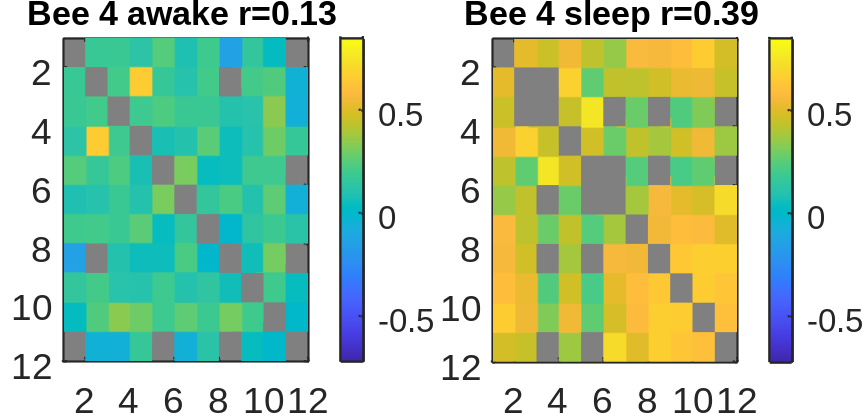
\includegraphics[width=0.8\textwidth]{exp-change-correlation}
  \caption{Correlation change between the activity of projection neurons activity averaged over glomeruli. Image from \cite{sleep-correlates}.}
  \label{fig:exp-change-correlation}
\end{figure}

The main hypothesis is that these changes are due to changes in connectivity between neurons and due to brain-wide changes in the structure of neurons' activity.
In particular, during sleep inhibitory GABAergic synapses reduce their strength \cite{gaba}.
The computational model will be used to investigate this as it allows to artificially change synapses' conductances and observe the effect on the activity of the system.
Moreover, currents with different shapes will be injected into the model to see whether they are able to generate the observed effect.

\section{Developing a computational model of the antennal lobe}
Developing a computational model of the antennal lobe is a necessary step to achieve the main objective of this work.
The model is a recurrent spiking neural network with a structure similar to the one of the biological antennal lobe.
Developing such a model presents several challenges, due to the complexity of the biological system and the length of the simulation necessary to collect meaningful data.\\
This complexity will be tackled in a number of ways.
The spatial complexity of the model will be addressed by developing a modular system, facilitating the manipulation of its parameters systematically.
The computational complexity of the problem is tackled by using genn \cite{genn}, a GPU-accelerated simulator, which allows to run the simulation in a reasonable amount of time.
Recent development in GPU architecture has made it possible to run large-scale simulations taking advantage of the parallelism potential of GPUs.
The library genn allows to transpile Python code into CUDA \cite{cuda} code, which is then compiled and run on the GPU, allowing for fast development and deployment times without loss of performance.
The developed code is then wrapped in a Docker container \cite{docker} and deployed to an HPC cluster, where it is transpiled and the simulation is run in a high-performance environment.
The data collected is then stored in a compressed binary form and used for a later analysis pipeline.
The entire pipeline is represented in figure \ref{fig:pipeline}.
This approach allows to run the simulation and the data analysis pipeline in a reasonable amount of time while maintaining the flexibility of Python code.\\
The data analysis pipeline will allow to extract the relevant features from the data and to compare them with the experimental data.
In particular, the focus will be on the activity pattern of the neurons of the antennal lobe, their correlation and how changes in the strength of the synapses and in the shape of the input will affect the neuronal computation undergoing in the olfactory system.


\begin{figure}
  \centering
  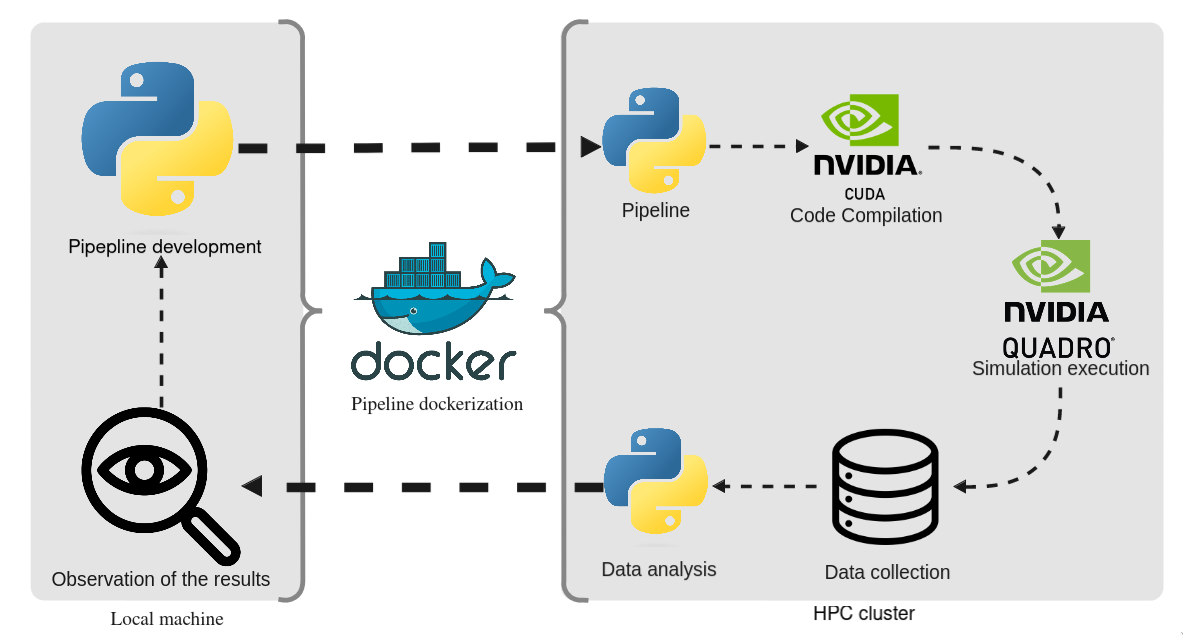
\includegraphics[width=0.8\textwidth]{pipeline}
  \caption{Visual representation of the development pipeline.}
  \label{fig:pipeline}
\end{figure}
